\chapter{Modeling human representational geometry}
\label{chap:modeling_human}

From a historical point of view, the success of RSA brought to many studies on ablation, plasticity, etc. Many researchers used it, but they started questioning whether it is a good model of human knowledge. In the following we are discussing different assumptions, in respect to artificial DNN.

\section{Background}
We have already seen in Chapter \ref{chap:concepts_categories} the most accepted representation of concepts, as categories, in psychology: semantic domains or categories (e.g. mammals, animals, dogs) are organized via features or dimensions that carry the relevant variance for the category (Classical view, Rosch and Mervis (1975), \cite{lake-2015-deep}).
We have also seen how we can have typicality effects in AI: entities (e.g. images, words) are described by feature values from which representational category effects emerge.

We can use AI systems as models of semantics (Section \ref{sec:kriegeskorte}): AI systems trained for image categorization or word embedding produce representations that reasonably approximate those of humans. Similarity between categories, as operationalized from human data, is well predicted by distances between objects in the AI model, where human similarity is quantified using brain/behavior and model similarity is quantified via Euclidean distances, inverse cosine, etc.
For prediction of human similarity judgments on images, they found 20 to 60\% of the judgments is modeled by the NN. While in MVPA the results are more complicated: these can predict activation in brain areas, but the correlation is just barely above the significance threshold.

\section{AI modeling of human representations}
Modeling human representations with AI is useful for many fields:
\begin{itemize}
    \item Psychology: AI models achieve human-like competence on different tasks. Because of their competence, they offer a \textbf{model of potential knowledge organization}. They can also offer \textbf{interpretability of human behaviour}: if we have an AI model that behaves as humans, we can study it to come up with valid hypotheses.
    \item Engineering: better prediction of human behavior, and improved AI-human alignment. For instance, to evaluate how good generated images are, similarity metrics are used. However this does not take into account the subjectivity of human brain.
    \item Computer science: understanding representations in neural networks.
\end{itemize}

There are three approaches:
\begin{itemize}
    \item \textbf{Default}: \textbf{use all DNN features} (all in the whole network, or all in a particular layer) as object-representation for modeling human data. This implicitly assumes that all features are relevant and equally important, for the alignment, for all concepts.
    \item \textbf{Reweighting}: \textbf{keep all features, but adjust the weights by finetuning}. It addresses mis-calibrated, human-relevant features by applying concept-specific adjustment of feature saliency for modeling human representations. This assumes that AI learns human-relevant features, but these are mis-calibrated.
    \item \textbf{Pruning}: \textbf{keep the weights unchanged but remove some features}, investigating modular structures in AI models. This assumes that the network develops a modular structure where information about different categories is represented in different subspaces (subsets of latent dimensions) within the model, i.e., knowledge about particular categories or concepts is stored in particular areas (``modules") in the AI model.
\end{itemize}

\subsection{Default approach}
Assuming two objects, $U$ and $V$, each with 3 features, \textbf{human similarity} can be defined using the \textbf{inner product} (or a related quantity), and approximated as follows:
\[
    Similarity(V,U) = V \cdot U = V_1 \cdot U_1 +  V_2 \cdot U_2 + V_3 \cdot U_3
\]
Note this is just an evaluation (no learning involved).

\subsection{Reweighting}
% \subsection[Reweighting]{Reweighting, \mandatory{peterson}}
The similarity is defined as the \textbf{weighted inner product} (or related measure), where the weights ($W_{1,2,3}$) are learned via regression and evaluated on out-of-sample data.
\[
    Similarity(V,U) = W_1 \cdot V_1 \cdot U_1 + W_2 \cdot V_2 \cdot U_2 + W_3 \cdot V_3 \cdot U_3
\]
This \textbf{involves learning} (via linear regression or other techniques). Learning the weights is far from easy, since the number of free parameters is extremely huge (regularization is needed), as weight solutions are category-specific.
\notedv \cite{peterson} proved that this approach generalizes well, outperforming the baseline (default approach), despite this being already high.\\

\boxl{\mandatory{peterson}\\ \textit{Evaluating (and Improving) the Correspondence Between Deep Neural Networks and Human Representations}}{
This study explores how well the representations discovered by DNNs align with human psychological representations of natural images, shows how they can be adjusted to increase this correspondence, and demonstrates that the resulting representations can be used to predict complex human behaviors such as learning novel categories.

Reweighting starts like RSA, by comparing the representations formed by deep neural networks to those of humans, i.e., similarity judgments (accordingly, the first experiment of the paper focuses on this comparison). Notice that a similarity function over a set of  pairs of data points corresponds to an implicit representation of those  points.\\

Firstly, they evaluate the performance of deep neural networks in predicting human similarity judgments for 6 categories of images (120 images each). They collect the human judgements as pairwise image similarity ratings (within each category) from human participants on Amazon Mechanical Turk, using a scale from 0 (``not similar at all") to 10 (``very similar"). The result is six $120 \times 120$ similarity matrices after averaging over individual judgments. They collect the activations of a DNN (they experiment with several models, here are the results of VGG only) in a feature matrix, with an image per row, that therefore has shape [$120 \times 4096$]. A similarity matrix $\mathbf{S}$, in which the entry $s_{ij}$ gives the human similarity judgements between images $i$ and $j$, can then be approximated by the matrix product $\mathbf{FF}^T$:
\[
\mathbf{S=FF}^T
\]
They assess the model performance in predicting human similarity judgments by computing the correlation between $\mathbf{S}$ and $\mathbf{FF}^T$, finding that the \textbf{raw deep representations provide a reasonable first approximation to human similarity judgments}.
}
\boxs{

To better understand how DNNs succeed and fail to reproduce the structure of psychological representations, they applied  two classic psychological tools: \textit{non-metric multidimensional scaling}, which converts similarities into a spatial representation (from relative distances of $n$ elements to a map of relative distances in 2 dimensions), and \textit{hierarchical clustering}, which produces a tree structure (dendrogram). They find that human representations exhibit highly distinguished clusters in the spatial projections and intuitive taxonomic structure in the dendrograms, neither of which is present in the DNN representations.\\

They procede exploring how DNN representations can be transformed to increase their alignment with psychological representations.
They augment the model of similarity judgments with a set of weights on the features used to compute similarity:
\[
\mathbf{S=FWF}^T
\]
where $\mathbf{W}$ is a diagonal matrix of dimension weights. the diagonal of $\mathbf{W}$, the vector of weights $\mathbf{w}$, can be expressed as the solution to a linear regression problem where the predictors for each similarity $s_{ij}$ are the (elementwise) product of the values of each feature for objects $i$ and $j$ (i.e., each row of the regression design matrix $X$ can be written as $\mathbf{F}_i \circ \mathbf{F}_j$, where $\circ$ is the Hadamard product). The similarity $s_{ij}$ between objects $i$ and $j$ is therefore modeled as
\[
s_{ij} = \sum_k w_k f_{ik} f_{jk}
\]
where $f_{ik}$ is the $k$\textsuperscript{th} feature of image $i$ and $w_k$ is its weight.

Freely identifying the $\mathbf{w}$ that best predicts human similarity judgments runs the risk of over-fitting, since the DNN generates thousands of features. To address this, they use L2 regularization on $\mathbf{w}$, penalizing models for which the inner product $\mathbf{w}^T\mathbf{w}$ is large.\\

The \textbf{new representations that emerge explain nearly twice the variance compared to raw representations} on all domains:

\begin{center}
    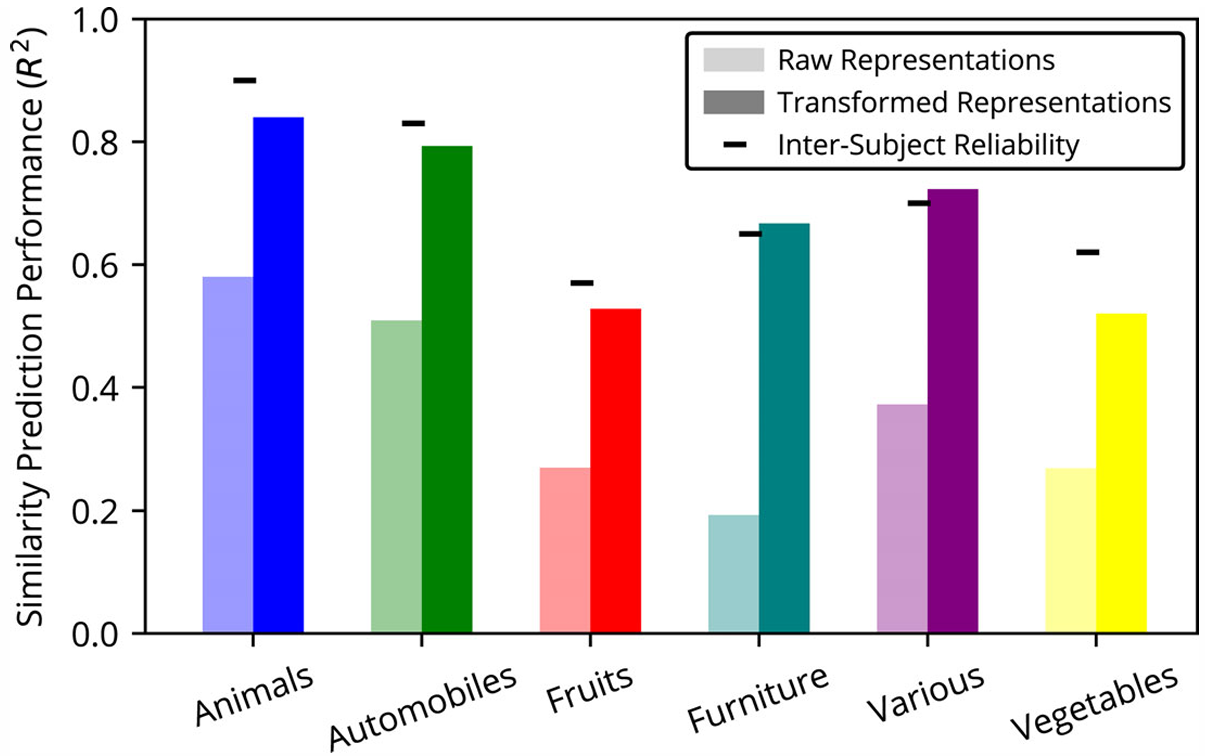
\includegraphics[width=0.5\textwidth]{images/sfft.png}
\end{center}

The stricter case of cross-validation titled ``CV control" explains the similarity judgements better than raw  representations. In this case no single images occurred in both training folds and test folds of cross-validation. However, for ``Transformed model", the exclusivity was in respect to pair of images.

The MDS and dendrogram plots for the transformed representations show a stronger resemblance to the original human judgments:

\begin{center}
    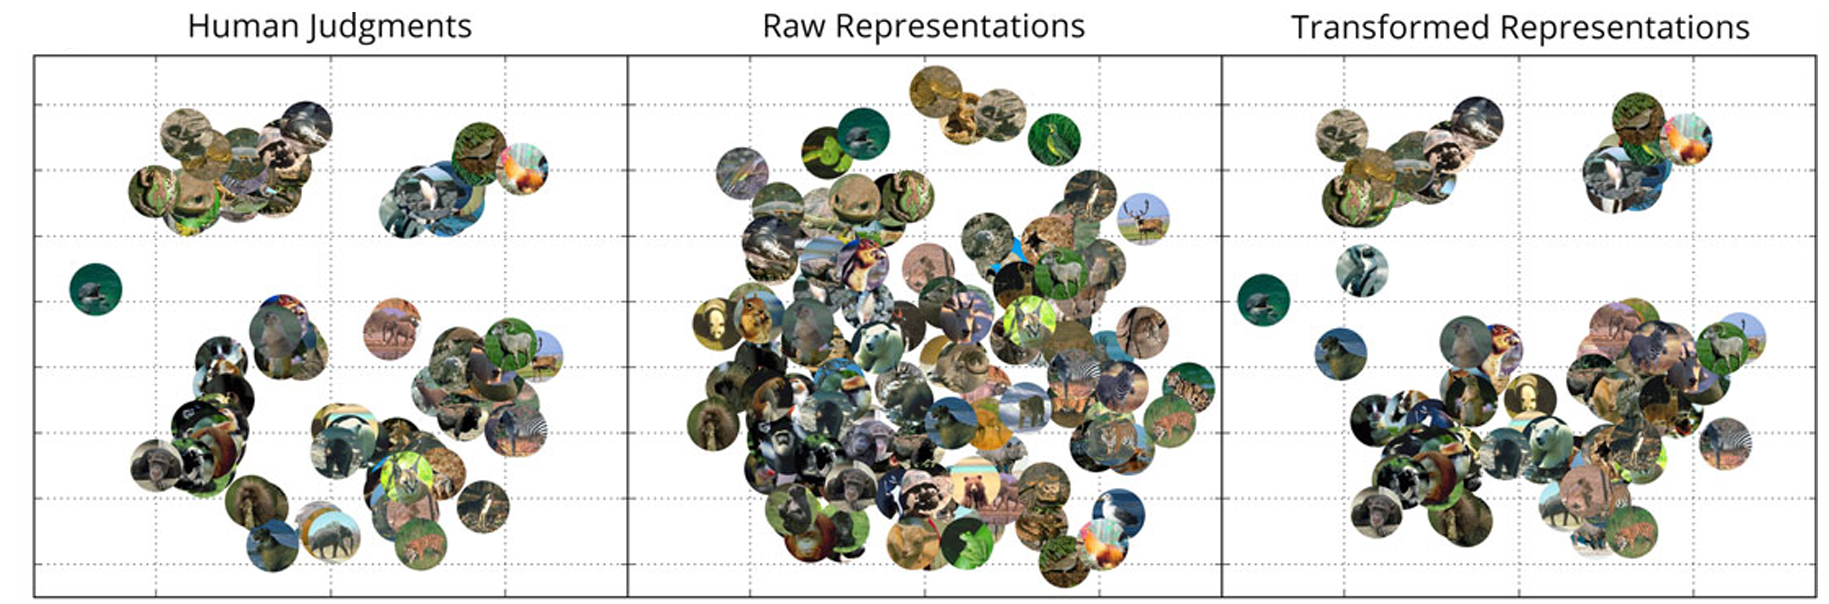
\includegraphics[width=0.75\textwidth]{images/reweighting.png}
\end{center}
}
\boxs{

\begin{center}
    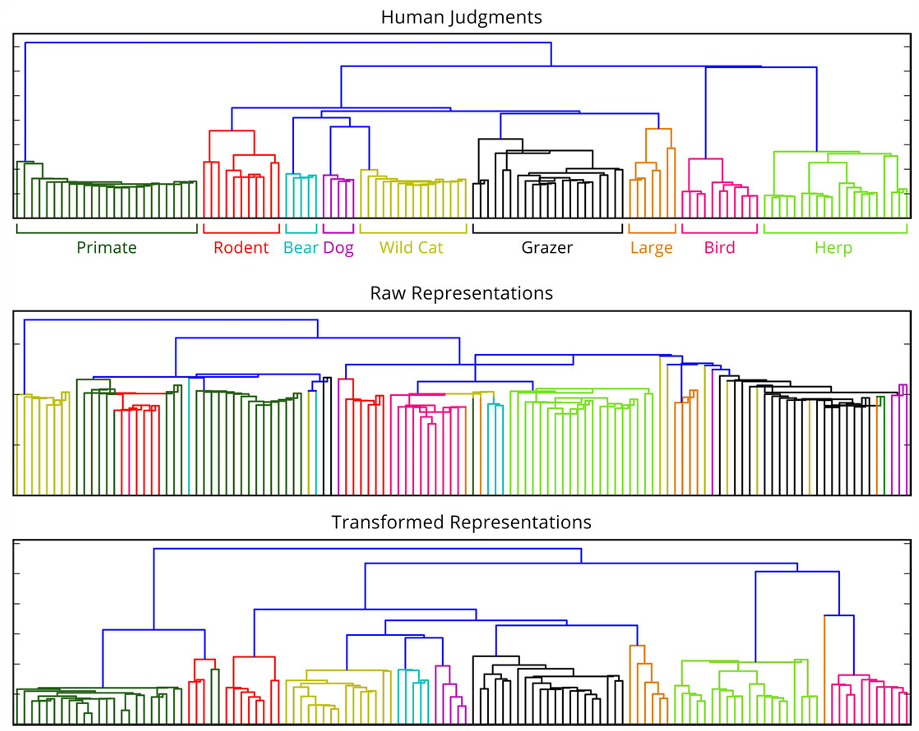
\includegraphics[width=0.55\textwidth]{images/reweighting_2.png}
\end{center}

The transformations learned are highly contingent on the domain and do not generalize well to others. However, it is possible to use the same adaptation method to produce a more robust transformation of the DNN representations for the purposes of predicting human similarity judgments. To do so, they learn a transformation using all six domains at once.

In conclusion, DNNs develop the correct basis set of features, just at the wrong level of saliency. Learning a reweighting of salience (transformed representation) improves prediction of human similarity judgments. The simple re-weighting of features, that the linear transformation  performs, can be viewed as an analogue to dimensional attention. The ability of transformed representations to generalise for new stimuli empowers studies on cognitive processes relying on such representations in the brain.
}

\subsection{Pruning}
Differently than reweighting, pruning assumes that DNNs \textbf{do acquire the relevant features at appropriate levels of salience}, but the \textbf{contribution of relevant features is diluted by irrelevant ones}. Pruning aims at identifying a \textbf{subset of features}, \textbf{per category}, improving prediction of human representations (i.e., that produces object-to-object distances that best match those produced from human behavior), e.g.:
\[
    Similarity(V,U) = V_2 \cdot U_2 + V_3 \cdot U_3
\]
By iterating over features and using \textit{Sequential Feature Selection} algorithms, supervised pruning learns a subset of features that \textbf{better predicts human judgments and generalizes to out-of-sample data}. It is supervised as it uses human judgments to choose which features to prune.

\boxc{Pruning at work: a toy example}{
Humans find Tigers more similar to Lions than to Pumas. The model representation is disaligned from human representation (as Tiger-Lion and Tiger-Puma distances are the same in the embedding space of the model).
We see that removing Y-Dimension brings the embedding space closer to human representation:
\begin{center}
    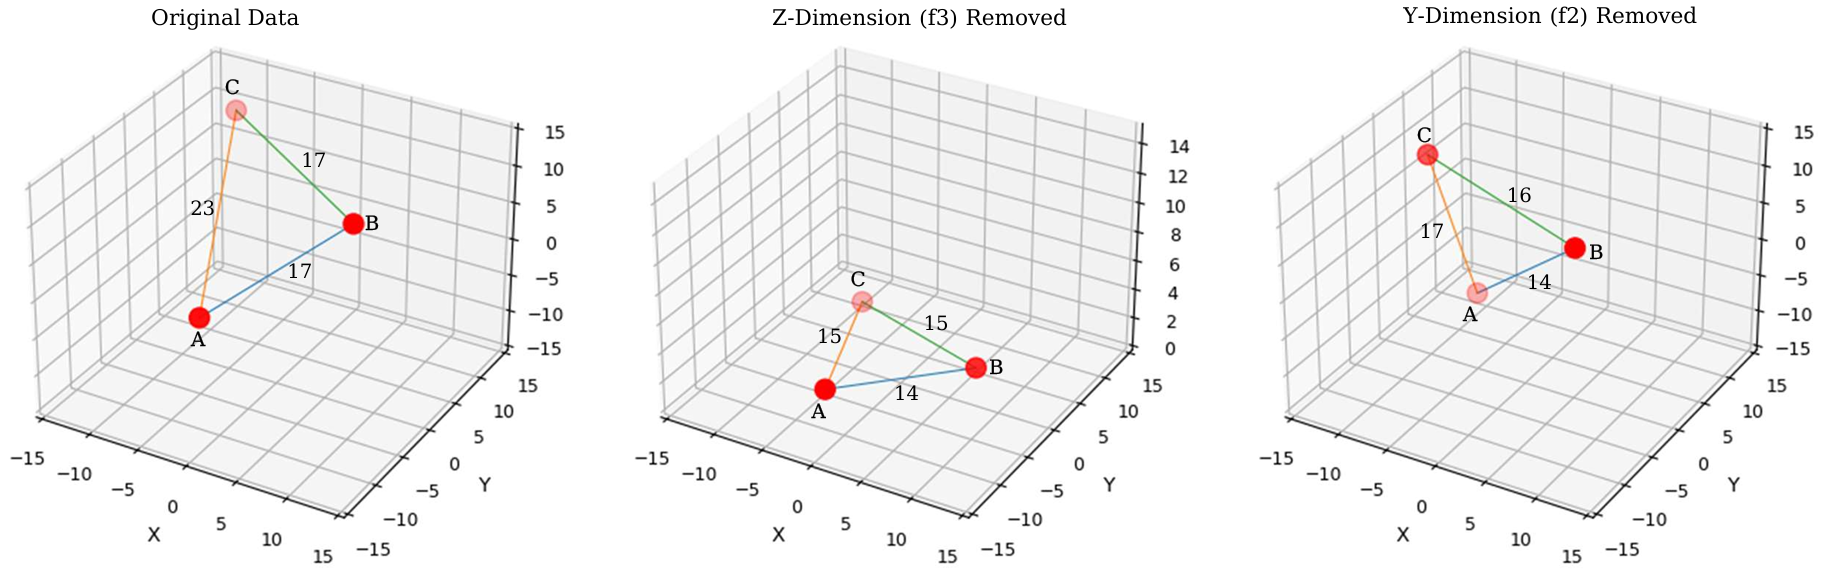
\includegraphics[width=0.9\textwidth]{images/pruning.png}
\end{center}
}
To summarize, pruning:
\begin{itemize}
    \item improves out-of-sample prediction accuracy for human similarity judgments of images, (higher RSA isomorphism);
    \item produces a more psychologically valid representational space;
    \item improves prediction of out-of-sample MVPA data (Brain RDMs).
\end{itemize}
Moreover, the feature-sets retained by pruning vary depending on the category guiding the pruning process, and these sets identify different subspaces (latent factors) in the feature space.
Pruning improves out of sample prediction of human similarity judgments for words and allows an interpretation of latent dimensions underlying word similarity judgments.

In the following we will go through a list studies on pruning to improve representational similarity between AI and Humans.

\boxl{\mandatory{TARIGOPULA202389}\\ \textit{Improved prediction of behavioral and neural similarity spaces using pruned DNNs}}{
They prune of a model that learns to predict human similarity judgments within 6 categories, each consisting of 120 images. In particular, they prune the penultimate layer of VGG19, which has 4096 nodes (features), and show that pruning outperforms other methods, including reweighting:
\begin{center}
    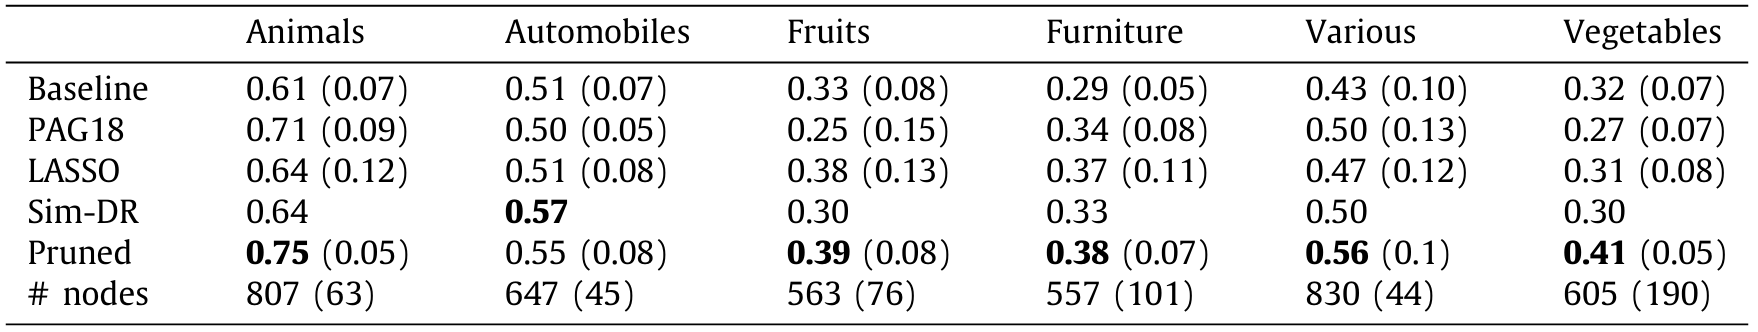
\includegraphics[width=0.8\textwidth]{images/tarigopula.png}
\end{center}
The number of nodes refers to how many nodes are retained by the pruning algorithm (e.g. for Animals 807 out of the original 4096).

They then proceed showing how pruning improves representational space for \textbf{out-of-sample image embeddings}. They first use a \textbf{different dataset} of Animal images and apply MDS (MultiDimentional Scaling); then they repeat but using only feature indices retained from pruning against the original experimental Animals dataset. In this second case, the animal types are better separated in the MDS representation (better clustering).

\begin{center}
    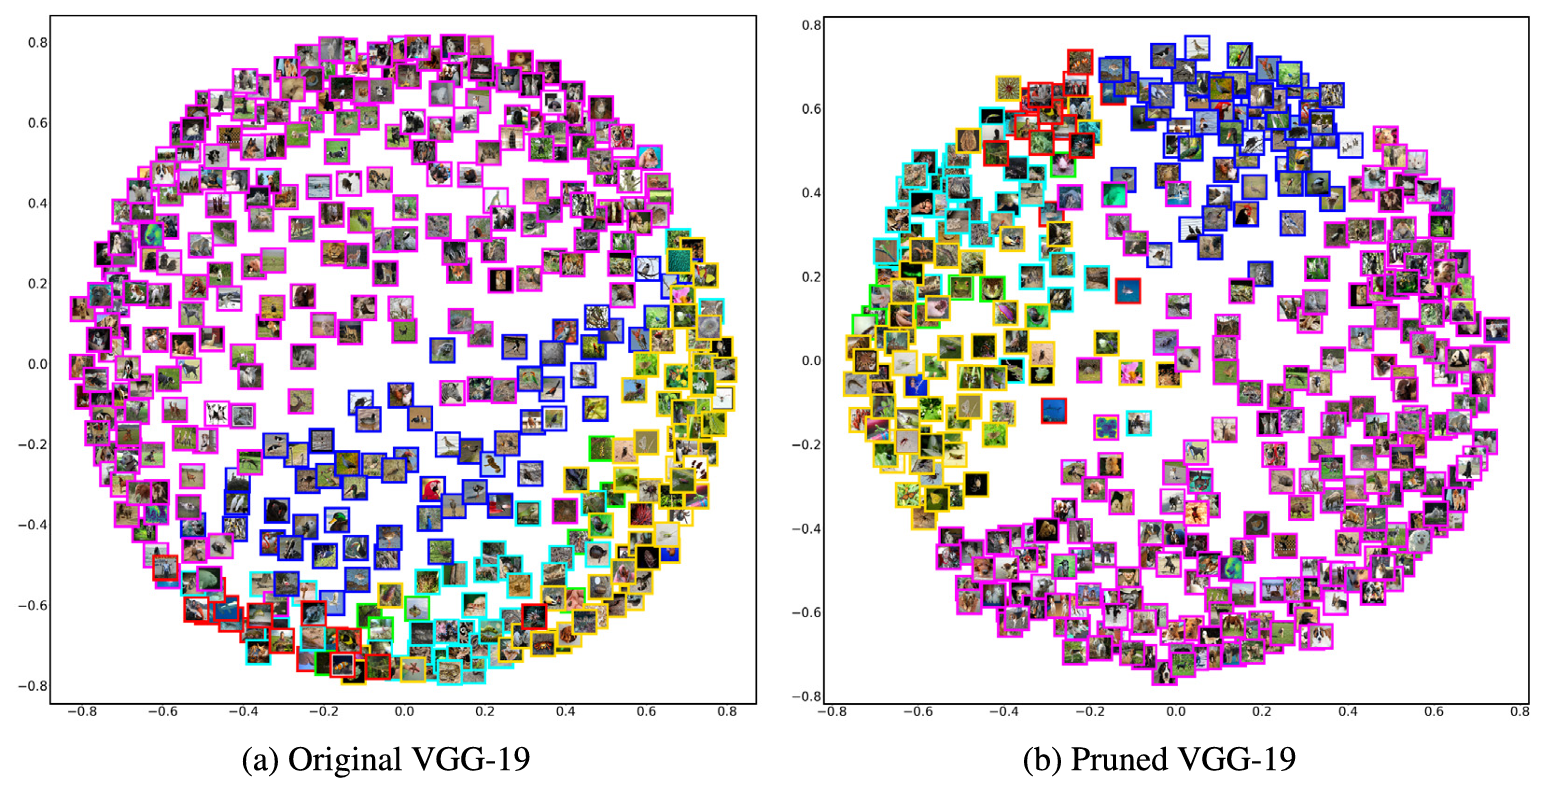
\includegraphics[width=0.65\textwidth]{images/mds.png}
\end{center}

Pruning also improves representational space for \textbf{out-of-sample brain data}. They use a dataset with two independent sets of 144 images. They produce RDMs from brain activity, per regions, then use RDMs to supervise pruning, and test on out-of-sample data, finding the prediction of brain-derived RDMs is improved.

\begin{center}
    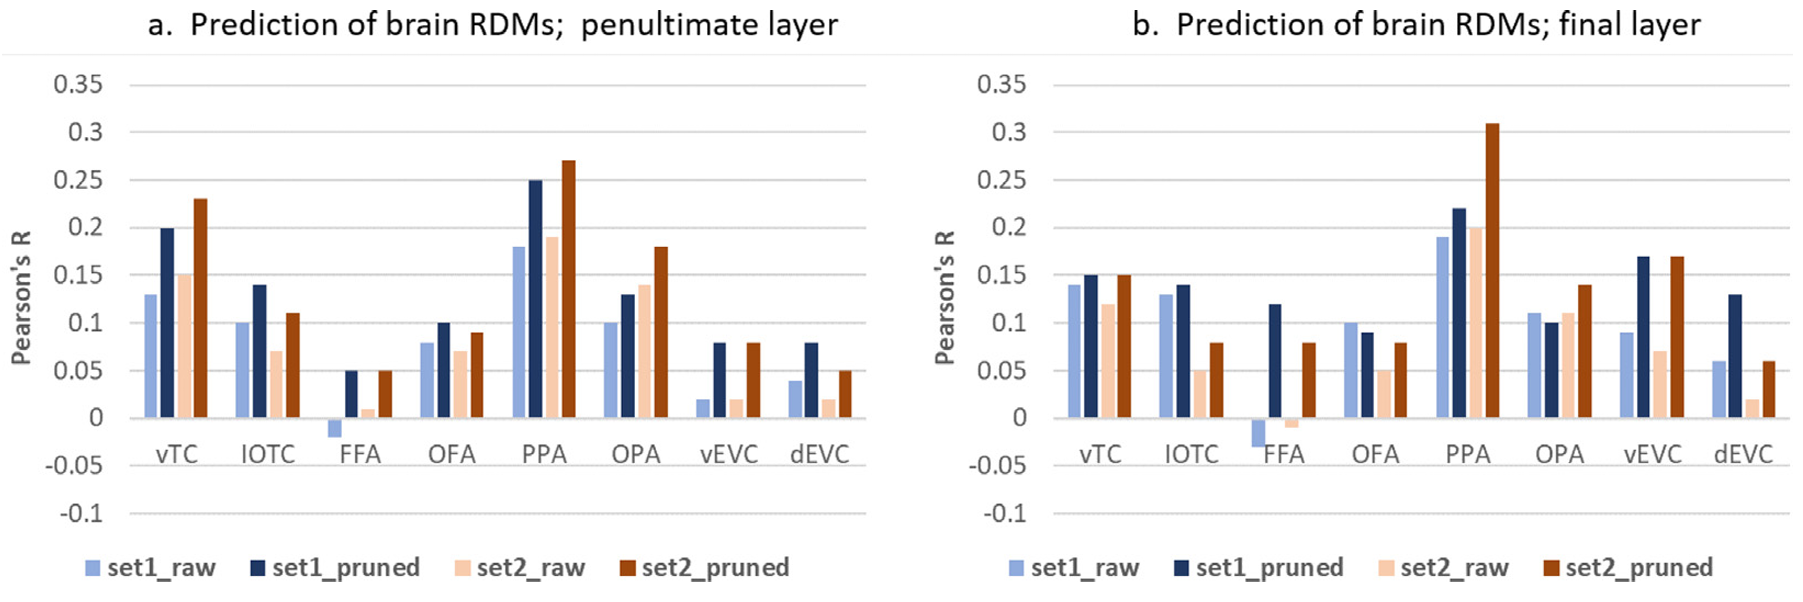
\includegraphics[width=0.9\textwidth]{images/tarigopula_2.png}
\end{center}
}

\boxl{Bavaresco et al. (unpublished)\\ \textit{Continuation of \cite{TARIGOPULA202389}}}{
They try to understand whether the different feature sets retained by pruning, for each class, are similar; and whether they code for different information. To measure the overlap between the (indices of the) features retained from the different category they use the Dice coefficient \notet:
\[
    DSC = 2 \cdot \frac{intersection}{union} 
\]
\osst{The Dice coefficient is also called \textit{Dice-Sørensen coefficient} or \textit{Dice similarity coefficient} (\textit{DSC}).}

They find the lowest value for $\langle Fruits,Automobiles\rangle$ (0.13) and the highest for $\langle Fruits,Vegetables\rangle$ (0.28). It is not surprising that the highest DSC value is between fruits and vegetables, which are indeed similar. However, in general, the overlap is quite low.
They find that just 1 out of 4096 feature is always selected for all 6 categories, meaning that there is not a ``core" set of features that is always retained.\\

To know if the selected features identify different information, they use a different dataset of 50k images. \textbf{Images are represented using only activations on the retained features} (6 different versions: 50k$\times807$; 50k$\times647$, etc.). For each of these derived embeddings they \textbf{identified the top-5 images that maximize activation on that set of features} (i.e., highest sum by row (in the matrix with inputs in rows and features in columns). They find that pruning-retained features, per category, are \textbf{maximized by images that exemplify the category}. This is consistent with the prototype theory.
Here is an example of the top-5 images for ``transportation" category:

\begin{center}
    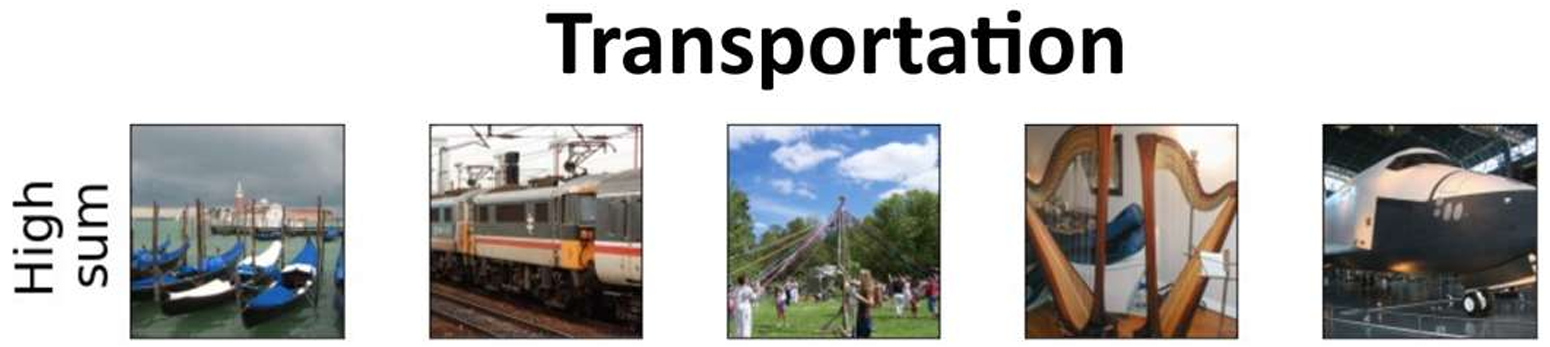
\includegraphics[width=0.5\textwidth]{images/bavaresco.png}
\end{center}

To have a more quantitative analysis, they apply PCA to each version (of the 6) and obtain the scores for the 50k images on the first Principal Component (this is needed since  the matrices are too large). Then the 50k PC1 scores are correlated across solutions (they get a score for each image). They conclude that \textbf{different retained sets select for different latent dimensions} (i.e., PC1 of similar categories encode for similar information).
}
\vspace{.5cm}
To summarize, human representations of concepts/categories are better approximated by AI models that are modified to reflect only the relevant variance dimensions, as indicated by specific subsets of features.
Practically, pruning via sequential feature selection is one way to identify these dimensions. It is competitive in learning human representations and allows to interpret the relevant lower dimensions.

\subsection{Pruning vs reweighting}
Vision DNNs trained to classify already provide a moderate approximation of human representational space.
Reweighting is emerging as a new technique to improve this match (useful for practical applications), and was interpreted to suggest that DNNs learn human-like filters, but at wrong levels of salience.

\textbf{Pruning outperforms reweighting} in learning prediction of human representational spaces, but also originates in a different perspective on the importance of DNN filters: the filters are effective at the learned levels of salience, but different datasets benefit from different combinations of filters. Pruning is also more \textbf{easily interpretable} as a regularization (data reduction) technique in context of explainable AI and provides insights into brain organization.

\boxl{Manrique et al. (2023)\\ \textit{ Enhancing Interpretability Using Human Similarity Judgements to Prune Word Embeddings}}{
They try to pring the same concepts of \cite{TARIGOPULA202389} to NLP. They define 8 categories as sets of 20-30 noun words each. They have human similarity judgments for all word pairs. The idea is to predict the test-set using all GloVe features, or GloVe feature-sets pruned from the training-set. The results show that \textbf{pruning improves out-of-sample prediction} using a \textbf{less than half of GloVe's 300 features}.
Notice that the features that are important for positioning objects with respect to each other are not necessarily important for classification, and vice versa.

For each solution they identify the retained feature indices and compute the DSC between pruned sets, which often results low (few of the GloVe features are never selected, and no feature is consistently selected). 
Some results make sense (fruit and vegetables have high overlap) but others do not (vehicles and fruit):

\begin{center}
    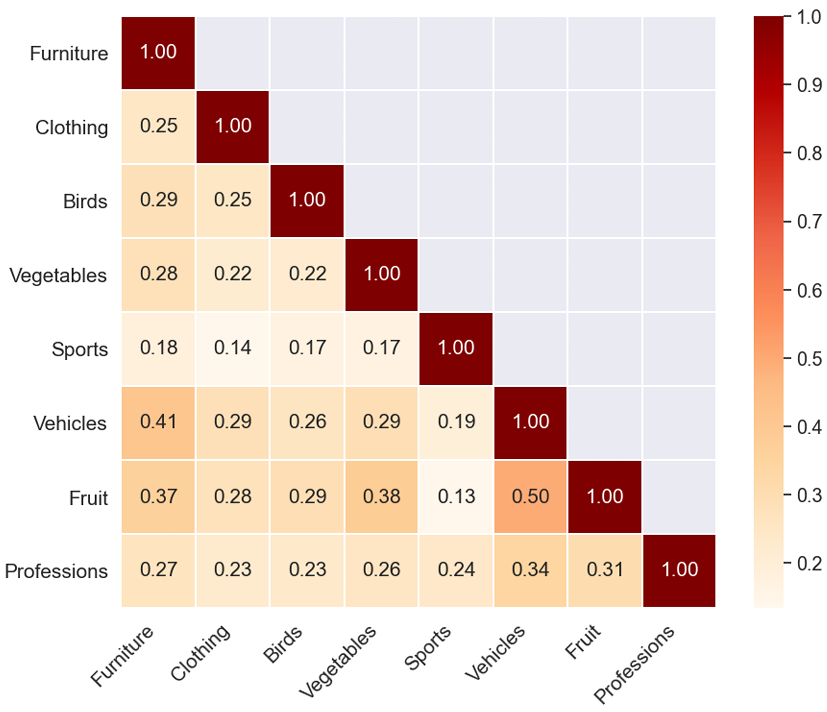
\includegraphics[width=0.38\textwidth]{images/dsc.png}
\end{center}

This is a problem for interpretability. So they try to understand what information is coded in a subset of features of a language model. Here an example with the ``sports" category is provided.
From previous pruning, 100 features out of 300 were retained, from these they take the following steps:
\begin{itemize}
    \item further reduce the dimensionality with PCA, retaining only the first PC
    \item rank sports by PC1 value
    \item for every word in the corpus, compute the co-occurence with each sport
    \item select the words whose co-occurence scores (in the form of PMI \notet) are correlated to the PC1 scores for each sport
\end{itemize}
\osst{PMI: Pointwise Mutual Information.}

The results suggest that human similarity judgments are sensitive to gender- and location-inclusiveness, and (relatedly) international reach.

\begin{center}
    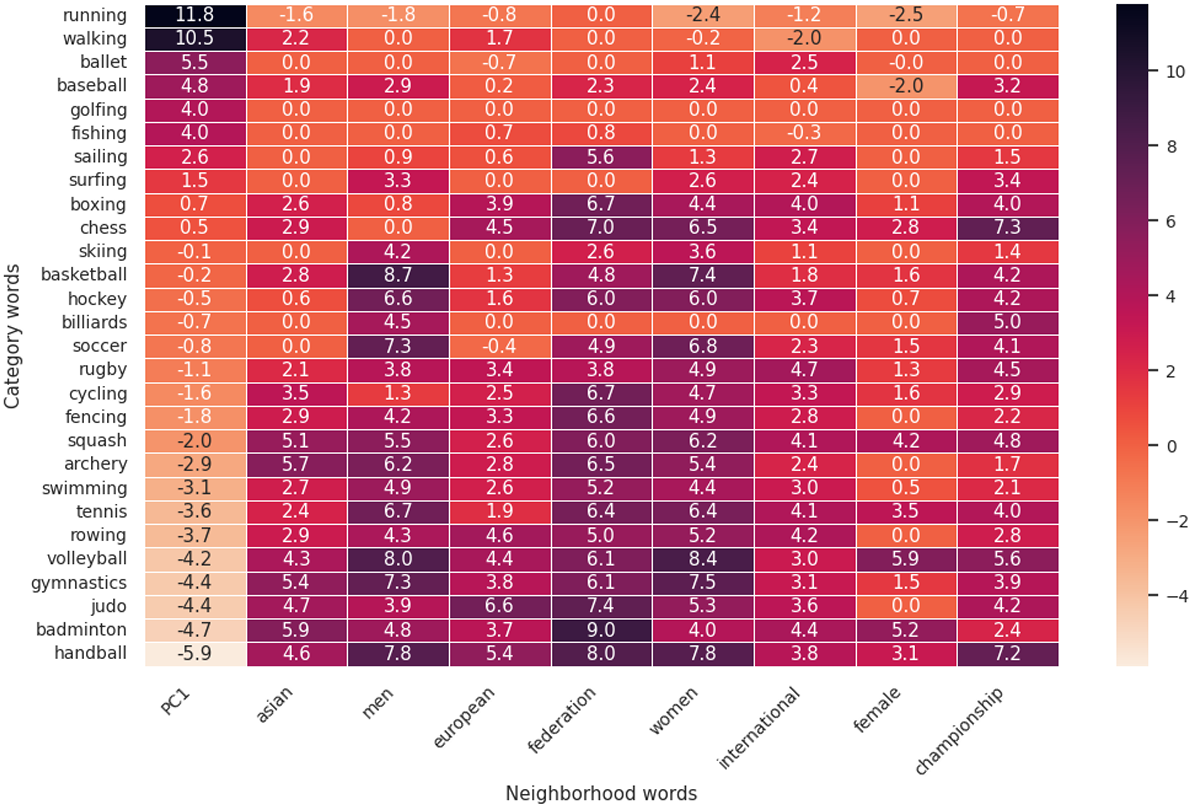
\includegraphics[width=0.68\textwidth]{images/sports.png}
\end{center}
}

\boxl{Bao et al. (2024)\\ \textit{Identifying and interpreting non-aligned human conceptual representations using language modeling}}{
This study tries to understand if \textbf{people of different groups represent words differently}. In particular they focus on English native speakers (blind vs sighted). They use 7 verb categories each containing 14 verbs and have \textbf{human similarity judgments} for all verb-pairs. The judgments \textbf{made by congenitally blind and sighted}. They train a model to prune GloVe embeddings to improve out-of-sample prediction, first for blind and then for sighted,so they can compute the DSC between the two subsets of retained features.

\begin{center}
    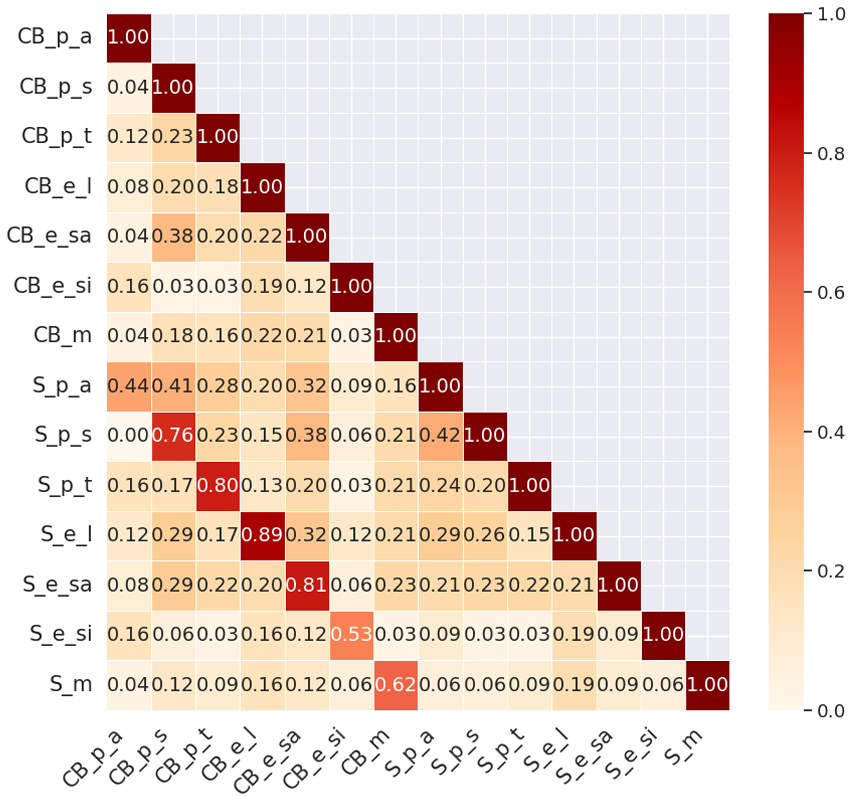
\includegraphics[width=0.55\textwidth]{images/bao.png}
\end{center}

They found that verbs describing emission of animate sounds (\texttt{e\_sa}, e.g. \textit{whine}) and light (e.g. \textit{blink}) have good concordance between retained features for blind (\texttt{CB}) and sighted (\texttt{S}). For others, such as perception sight (\texttt{p\_s}, e.g. \textit{see}, \textit{look}), a lower concordance is found.
}
\vspace{.1cm}
\section[Why pruning works]{Why pruning works\\ \textit{Network Trimming: A Data-Driven Neuron Pruning Approach towards Efficient Deep Architectures}\\ \mandatory{hu2016network}}
Extremely sparse matrices produced by top layers of neural networks indicate that empirically designed networks are heavily oversized. Many neurons in a CNN have very low activations, no matter what data is presented. Such weak neurons are highly likely to be redundant and can be excluded without damaging the overall performance. Their existence can only increase the chance of overfitting and optimization difficulty.

\begin{wrapfigure}[12]{r}{0pt}
  \centering
  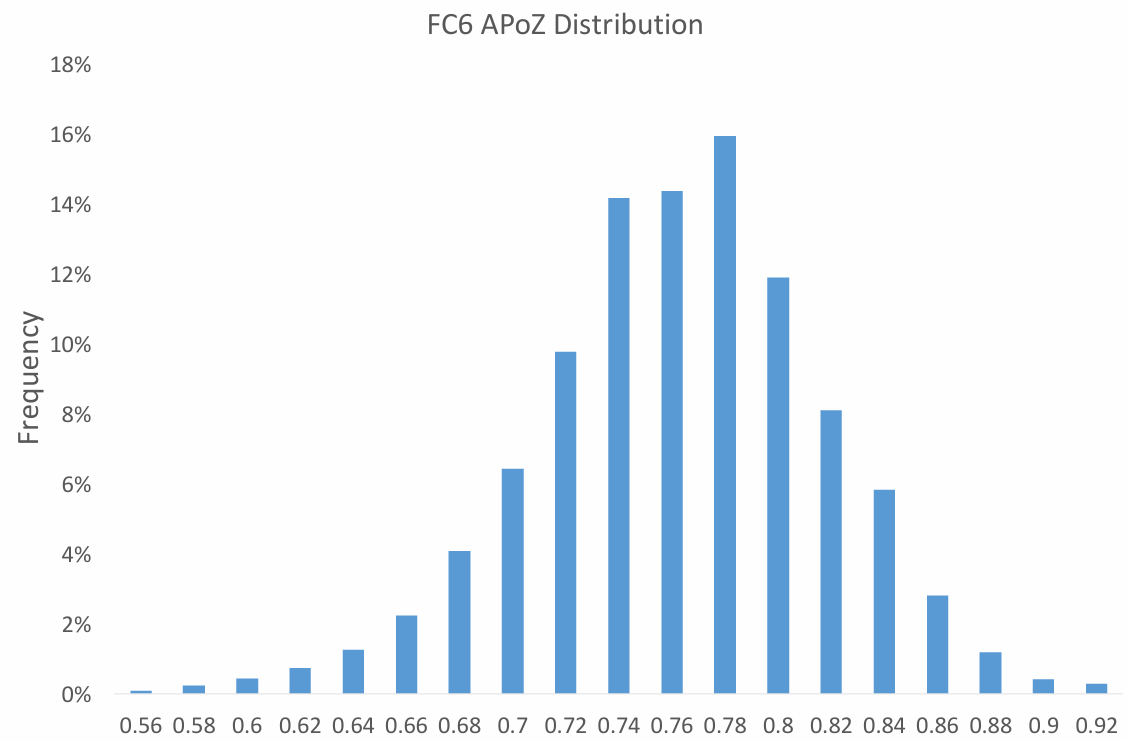
\includegraphics[width=0.41\textwidth]{images/apoz.png}
  \caption{\textit{FC6} layer \textit{APoZ} distribution.}
  \label{fig:apoz}
\end{wrapfigure}

They define the \textit{Average Percentage of Zeros} (\textit{APoZ}) of a single neuron as the percentage of zero activations of that neuron after the ReLU mapping. They use the layer as the unit of analysis (rather than the single neuron), so the analysis is collapsed across all neurons in a layer. The \textit{APoZ} of the $c$\textsuperscript{th} neuron in $i$\textsuperscript{th} layer is defined as:
\[
APoZ_c^{(i)} = APoZ(O_c^{(i)}) = \frac{\sum_k^N \sum_j^M f(O_{c,j}^{(i)}(k)=0)}{N\times M}
\]
where $f(\cdot) = 1$ if true, and $f(\cdot) = 0$ if false, $M$ denotes the dimension of output feature map of $O_c^{(i)}$, and $N$ denotes the total number of validation examples. Therefore $N\times M$ is the maximum number of activations.\\

The results tell that the redundancy is mainly in the deeper convolutional layers and the fully connected layers. They find more than 600 neurons with $APoZ > 90\%$ (Figure \ref{fig:apoz}).
To understand if high-$APoZ$ neurons are effectively redundant, they implement a neuron-pruning approach. After training to criteria, they remove all weights to and from high-$APoZ$ nodes (i.e., they remove these nodes from the network). They then re-initialize the network with the last set of weights (prior to pruning) and retrain to criteria (i.e., they fine-tune the pruned network).

\begin{figure}[!ht]
    \centering
    \captionsetup{width=.8\linewidth}
    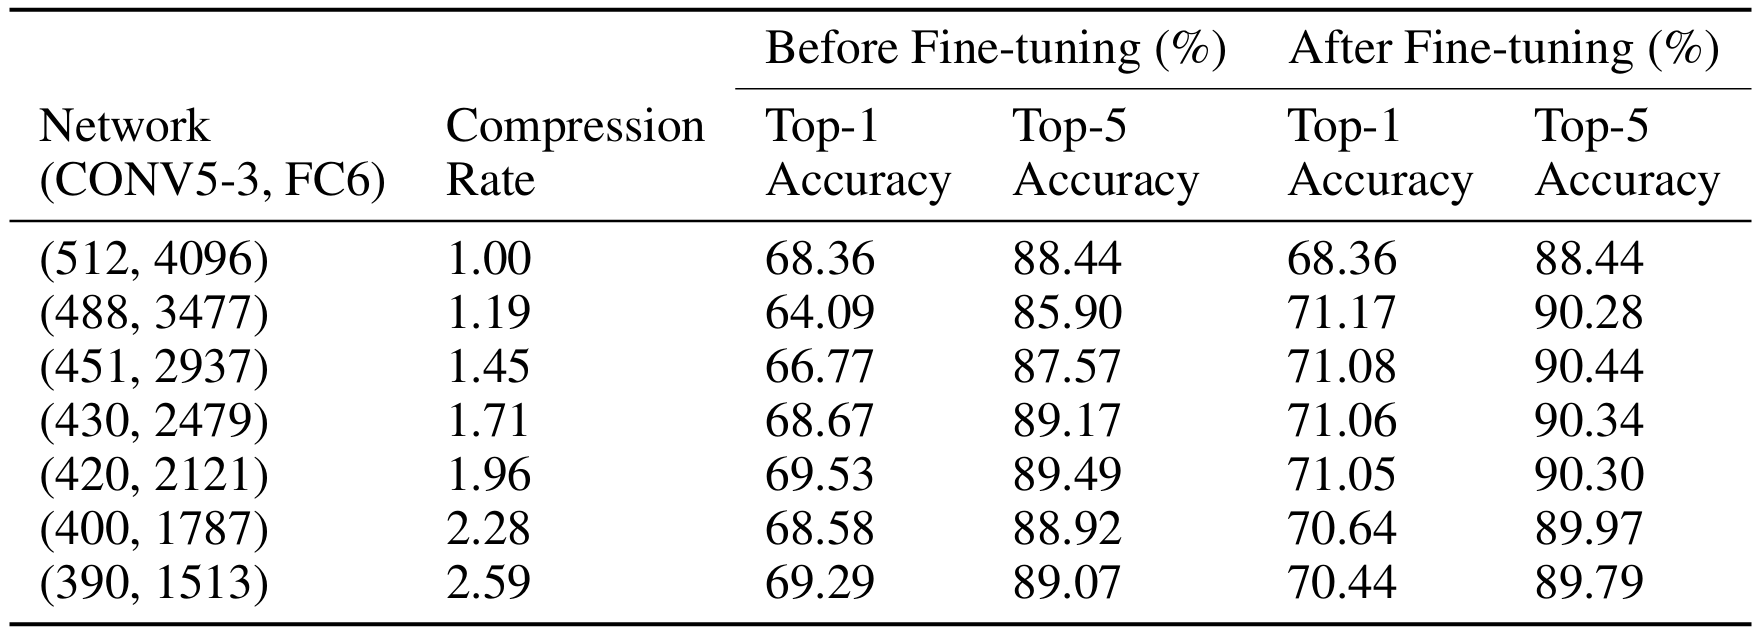
\includegraphics[width=0.65\linewidth]{images/trimming.png}
    \caption*{Example of trimming nodes in \textit{CONV5} and \textit{FC6} layers. We have to be aware that a column that is made of all 0s (i.e., a 100\%-\textit{PoZ} node) might still impact the representational geometry (object-similarities) if specific distance measures are used (see Section~\ref{sec:redundancy}).}
    \label{fig:trimming}
\end{figure}

\subsection{Redundancy and representational geometry}
\label{sec:redundancy}
For a given dataset, a 100\%-\textit{PoZ} feature does not provide discriminating information between objects. It may  serve to separate objects in this dataset from others. However, these features \textbf{do contribute to pair-wise similarity} estimations, i.e., estimation of object-similarity (cosine, Pearson).
Truong and Hasson (unpublished) try to answer the following questions:
\begin{itemize}
    \item How do these features contribute to a DNN's  Representational Dissimilarity Matrix (RDM)? 
    \item Can their removal improve prediction of human similarity judgments?
\end{itemize}

Figure \ref{fig:poz} shows how around 20\% of nodes in MNIST and CIFAR-10 have $PoZ>0.70$, while very few have $PoZ>0.95$.\\

\begin{wrapfigure}[13]{r}{0pt}
  \centering
  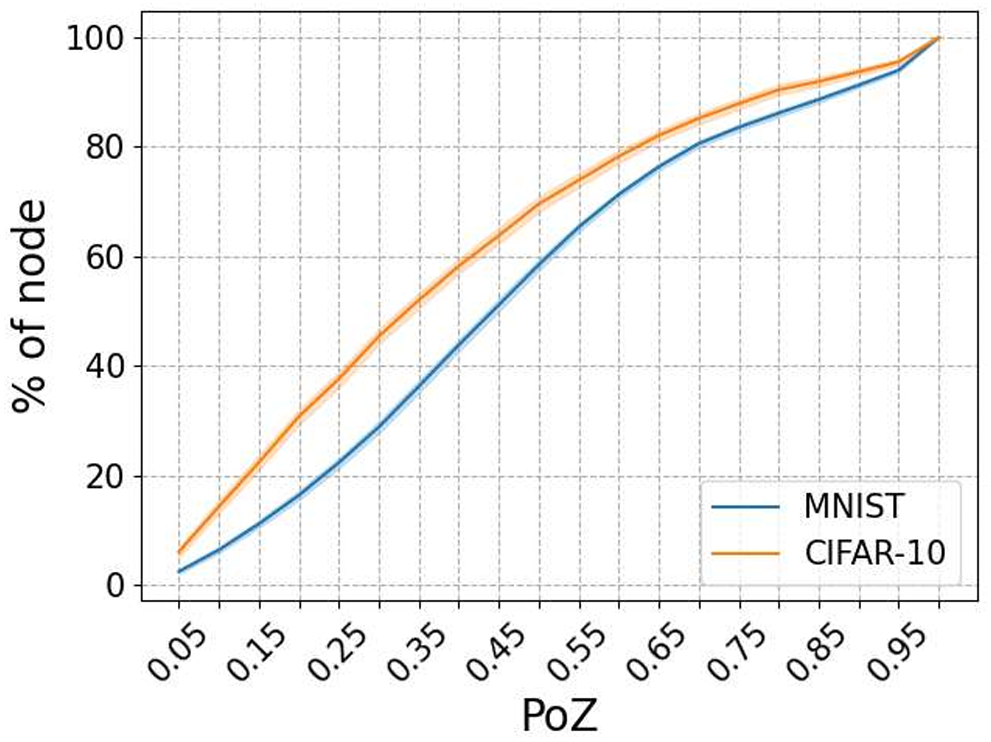
\includegraphics[width=0.35\textwidth]{images/poz.png}
  \caption{Percentage of nodes with a \textit{PoZ} lower than the given value.}
  \label{fig:poz}
\end{wrapfigure}

To answer the first question, they define the representation of the full network, and get the object-by-object similarity matrix (RDM), that will be used as reference. Then, they compute the RDM with just a small subset of features, the ones with lower \textit{PoZ}, and compare it with the original RDM (using Person $R^2$). They progressively insert features from low to high \textit{PoZ} (i.e., from the most informative features to the least ones) and repeat the steps. The results (Figure \ref{fig:poz_2}) show that it is possible to use just a subset of the original features, using the nodes with a \textit{PoZ} lower than $\sim35\%$, to approximate the representation of the original network.\\

They also try to understand what other nodes (those with the highest \textit{PoZ}) encode for. They experiment in the other direction, i.e., inserting features from high- to low-\textit{PoZ}. The results (Figure \ref{fig:poz_3}) show that these nodes are not random, nor they encode noise. They can indeed approximate the full network: the lowest 20\% already produces $R^2>0.6$ for CIFAR-10. This means \textbf{relevant information is coded in the network in a redundant way}.


\begin{figure}[!ht]
    \centering
    \captionsetup{width=.8\linewidth}
    \begin{subfigure}{.49\textwidth}
        \centering
        \captionsetup{width=.8\linewidth}
        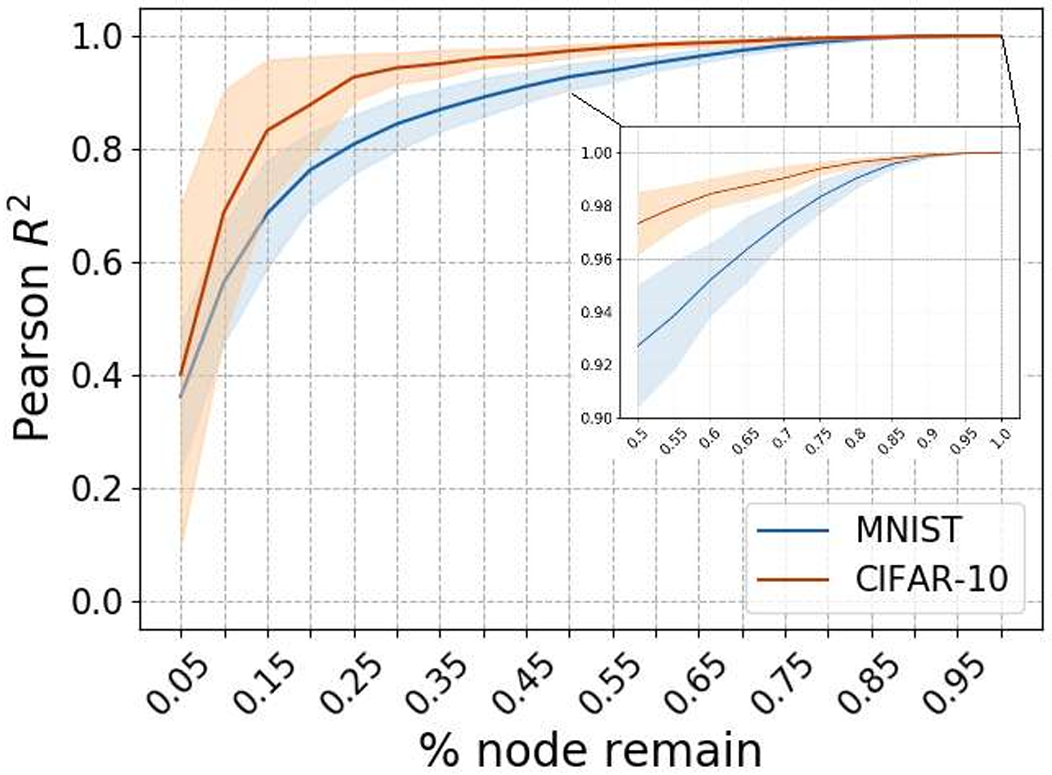
\includegraphics[width=.7\linewidth]{images/poz_2.png}
        \caption{Subset increased progressively from \textbf{low- to high-}\textit{PoZ} features.}
        \label{fig:poz_2}
    \end{subfigure}
    \begin{subfigure}{.49\textwidth}
        \centering
        \captionsetup{width=.8\linewidth}
        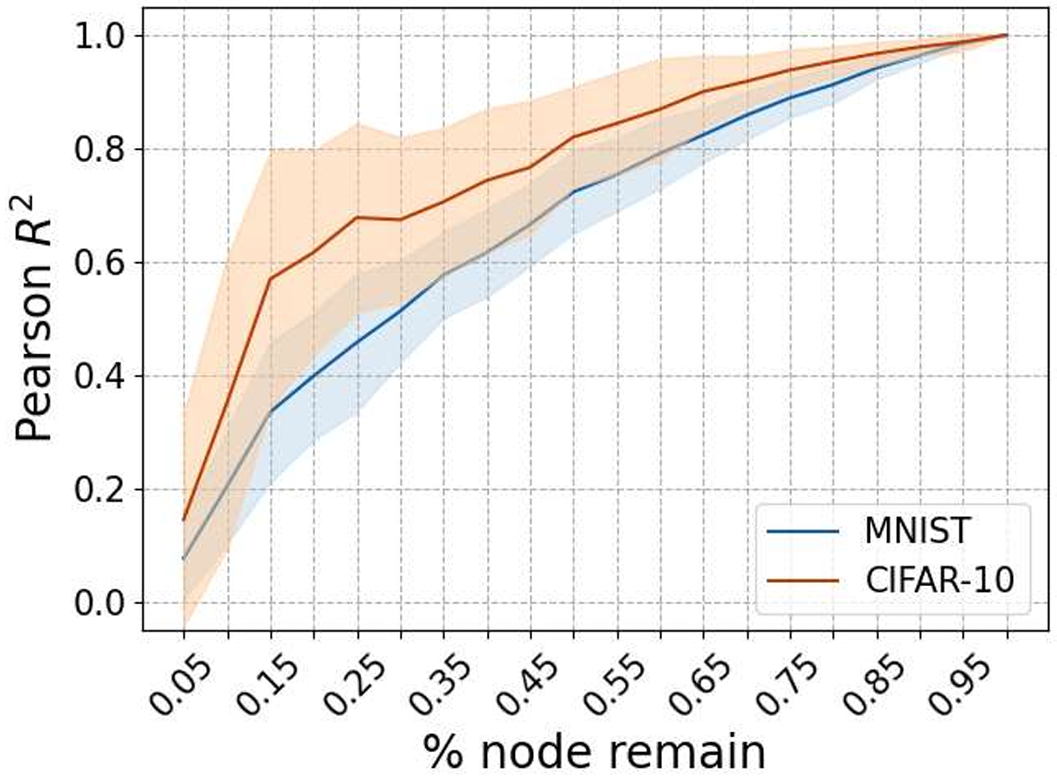
\includegraphics[width=.7\linewidth]{images/poz_3.png}
        \caption{Subset increased progressively from \textbf{high- to low-}\textit{PoZ} features.}
        \label{fig:poz_3}
    \end{subfigure}
    \caption{Similarity between the RDMs form a subset of features and the RDM got from the original embedding (all features).}
    \label{fig:poz23}
\end{figure}

\details{Adversarial attacks}{
When we prune a network we have to be aware that it becomes less robust to adversarial attacks, since the \textbf{embedding space becomes less sparse}, so that the \textbf{classes are closer to each other}.
}

\begin{wrapfigure}[13]{r}{0pt}
  \centering
  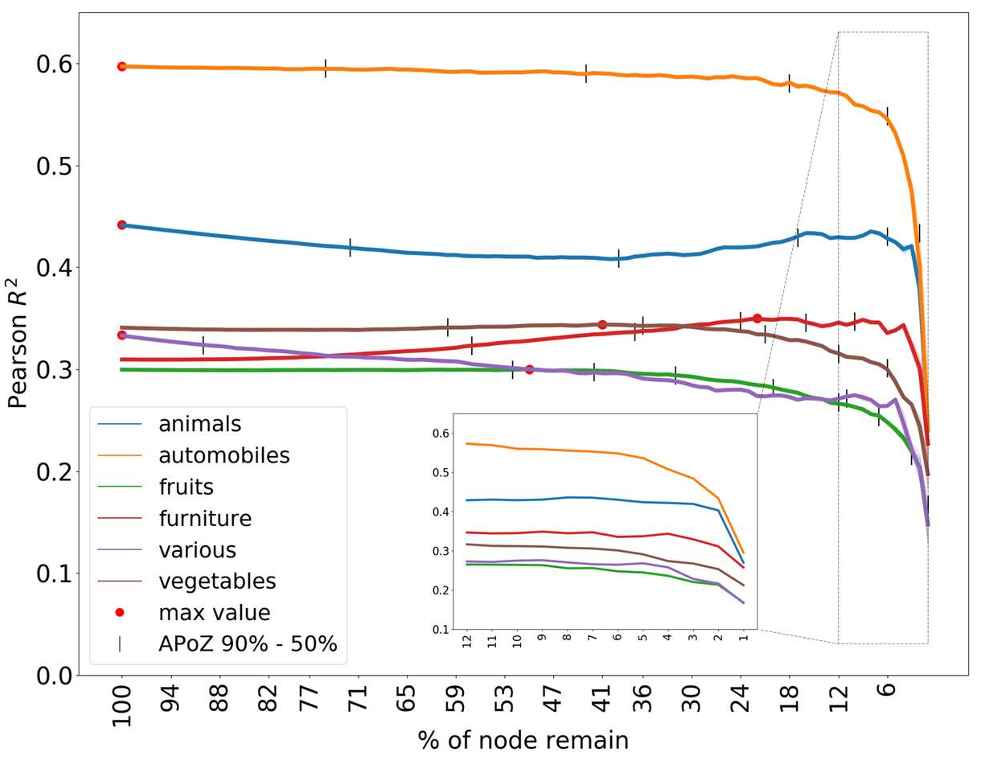
\includegraphics[width=0.45\textwidth]{images/apoz_4.png}
  \caption{Trimming using \textit{APoZ} and evaluating \textit{2OI} against human judgments.}
  \label{fig:apoz_4}
\end{wrapfigure}

To answer the second question they evaluate the \textit{APoZ}-based pruning and its impact on prediction of human similarity judgments. Features are removed sequentially from high-to-low \textit{PoZ} and \textit{2OI} (second-order interaction) is computed between human similarity judgments and the (pruned) model RDM.
The approximation of human similarity judgements starts dropping significantly only when we use less than 6\% of original features (Figure \ref{fig:apoz_4}).
We can notice that by removing sparse features, for the category of ``furniture", the approximation of human judgements increases until we use 30\% of the original features only. So, for ``furniture", sparse features actually contain noise.

